% version 1

\documentclass[10point]{article}

% prelude

\usepackage{fancyvrb}
\usepackage{graphicx}
\usepackage[pdftex, backref, colorlinks, bookmarksnumbered=true]{hyperref}

\DefineVerbatimEnvironment{code}{Verbatim}{}

\newcommand{\highlight}[1]{\colorbox{yellow}{#1}}
\newcommand{\highlighttt}[1]{\highlight{{\tt#1}}}

\long\def\ignore#1{}

\begin{document}

\title{Visuals Report}
\author{Callum McColl\\
	    Andrew Paroz}
		
\maketitle

\begin{abstract}
We did stuff. And more stuff, then stuff happened.
\end{abstract}

\tableofcontents

\listoffigures

\section{Introduction}
The goal of this project was to create a program that could compile, execute and displaye a C program. It could then be used to go step-by-step through a C program in order to show how the memory and registers are effected by each line of C code. In order to learn functional programming and Mash as a template, this program was created using Haskell. The project could be divided into 5 separate sections, the C parser, the assembly parser, C to assembly code generation, the emulator and the GUI. These were then allocated to three groups, one group would create the C Parser, another the Assembly Parser and Symbol Table, and the last group the Emulator and GUI. The Code generation which converts a C Parse tree to an Assembly Parse tree was not assigned to any group. A diagram of this can be see in Figure \ref{fig:ProjectDiagram}.

\begin{figure}[h]
\centering
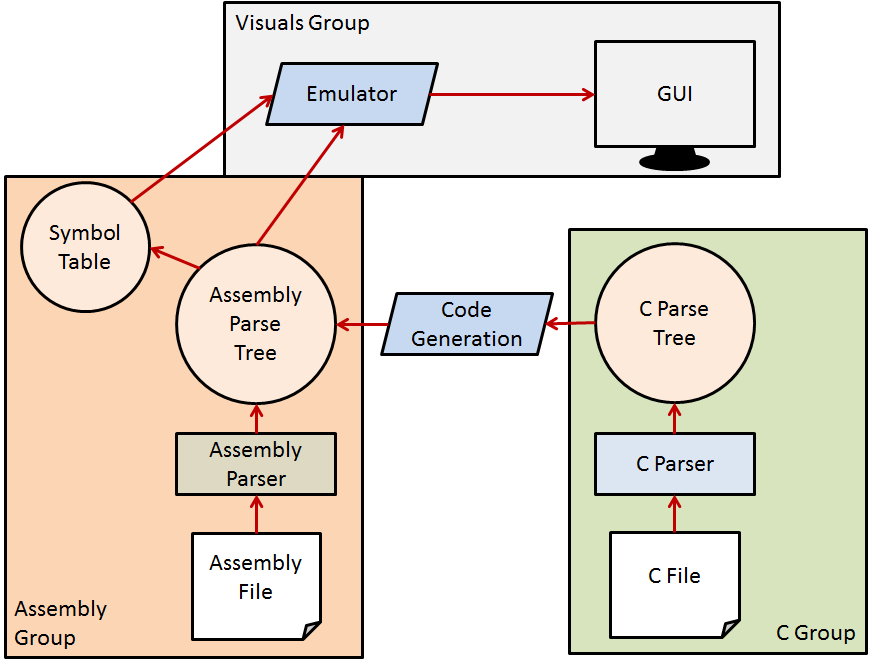
\includegraphics[width=300px]{ProjectDiagram}
\caption{Project diagram showing all the main parts and group allocations.}
\label{fig:ProjectDiagram}
\end{figure}

The program that this project created is to be used as a learning tool to help teach C programming. C is a difficult language when starting as there are multiple ways to do the same thing in the language, but some ways are more 'right' than others. The compilers can also be very lenient and compile and run code that is not correct, leading to problems where code ends up running differently on different systems. By having a program that can go step-by-step through a C program, it will be much easier to show where errors are, and explain to students why a program is acting in that way.

Obviously the C language is very vast, so only a small subset was chosen to be implemented for this project. All variables are either an Int or a pointer, there are no structs and everything must be contained within a single file. This allowed the assembler and emulator to be much simpler and made it possible to complete in the time we had.

Our group was the Visuals Group and was assigned to create the Emulator and GUI. Our project was significantly different from the other two groups which were creating parsers. In general, Callum was responsible for creating the GUI and Andrew created the Emulator and Environment. There was overlap between those sections when designing the programming interface for the emulator and environment, however most of the work was separate. Since the emulator uses an assembly parse tree, we also had to work with the group creating that in order to connect them together.

- ? More ? Maybe not.

\section{Process and Design}
Describe process / design

\subsection{Process}

As state previously Andrew was responsible for the Emulation and Callum was responsible for the GUI.  In order to easily share and work together a Git repository was set up.  This was essential as the application needed to be tested on Windows, Unix and Posix and each group member only had access to a subset of these platforms.  Therefore there were many times in the project where a group member would ask the other to pull the repository and verify that the behaviour exhibited by the program was correct.

Another benefit for using the repository was that it gave everyone developing the latest changes so it was known immediately if something that the other had changed had inadvertently affected the others work.  Overall the Git repository gave each developer the freedom to work individually without the worry of having to merge two separate implementation at a later date.

\subsection{Emulator}

\subsection{Graphical User Interface (GUI)}
\subsubsection{Cross-Platform GUI Solution}
The first task of our group was to determine how we would create a GUI using Haskell that could be completely cross-platform. Two methods were initially recommended, using Haskell to generate a HTML page that displayed everything, or using the GTK3 Hakell library to create an application window.

The first test was using a HTML page with a small amount of JavaScript to make it interactive. A screenshot of the example page can be seen in figure \ref{}. The idea was that once a program was compiled, it could generate this page with the all the program states loaded in as data. By using HTML, this file could then be opened on any system and the program could be looked at again without needing to be recompiled. However, it also had the huge drawback that the HTML page could not communicate with the emulator, which was too big a drawback for this project.

The next step was to test GTK3, and an example application was also made for it. This test program used Glade to structure the application window and GTK3 to draw it to the screen. A screenshot of the test program can be seen in figure \ref{fig:GTK3Test}. As a demo, it had very limited interactivity, allowing you to  step through a handwritten list of program states and nothing could be modified. It did demonstrate that GTK3 would indeed be suitable for the project, however the use of Glade to position elements on the window was not very useful as most of the windows ended up being built using code.

\begin{figure}[h]
\centering
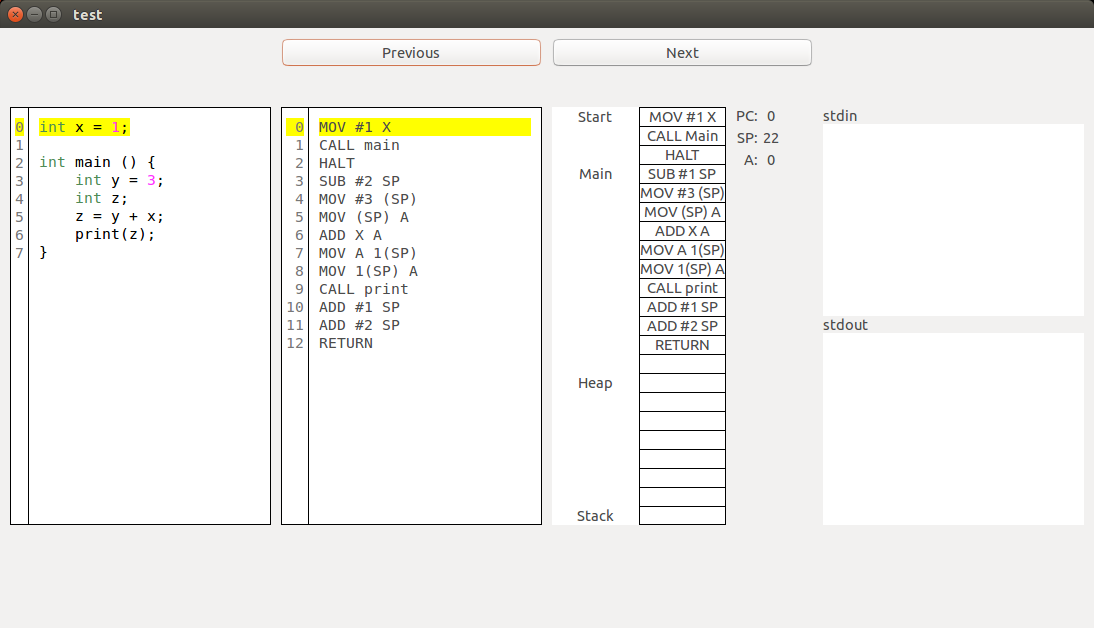
\includegraphics[width=300px]{GTK3TestScreenshot}
\caption{Screenshot of GTK3 test program.}
\label{fig:GTK3Test}
\end{figure}

\subsubsection{The Final Product}
While using Glade supplied a very nice proof-of-concept implementation, it became quite difficult to manage the dynamic nature of the program.  Therefore it was decided that attempting to complete the project using Glade was dropped for an entirely code based approach.

The final product follows from the proof-of-concept implementation but does of course emulate the assembly source code that it is given.  Unfortunately the C parsing was not completed so it was decided to abandon the C frame which is shown in the proof-of-concept implementation for more screen real estate.  The GUI has a main menu bar at the top which can be used to open other assembly source files.  Below the menu is a tool bar which presents play, stop, previous and next buttons.  This allows us to modify the assembly code and then run it much like other IDE's allow you to do.  Figures \ref{fig:screen_shot} and \ref{fig:screen_shot_running} show the final product when the assembly is editable and when it is begin emulated.

The GUI runs in two states.  Firstly when the GUI first launches it is in "edit" mode.  This means that the assembly source code and stdin are editable.  Once the user wants to run the emulation they then press the "play" button.  This runs the emulation.  The user is then able to step through the program.

\begin{figure}[h]
    \centering
    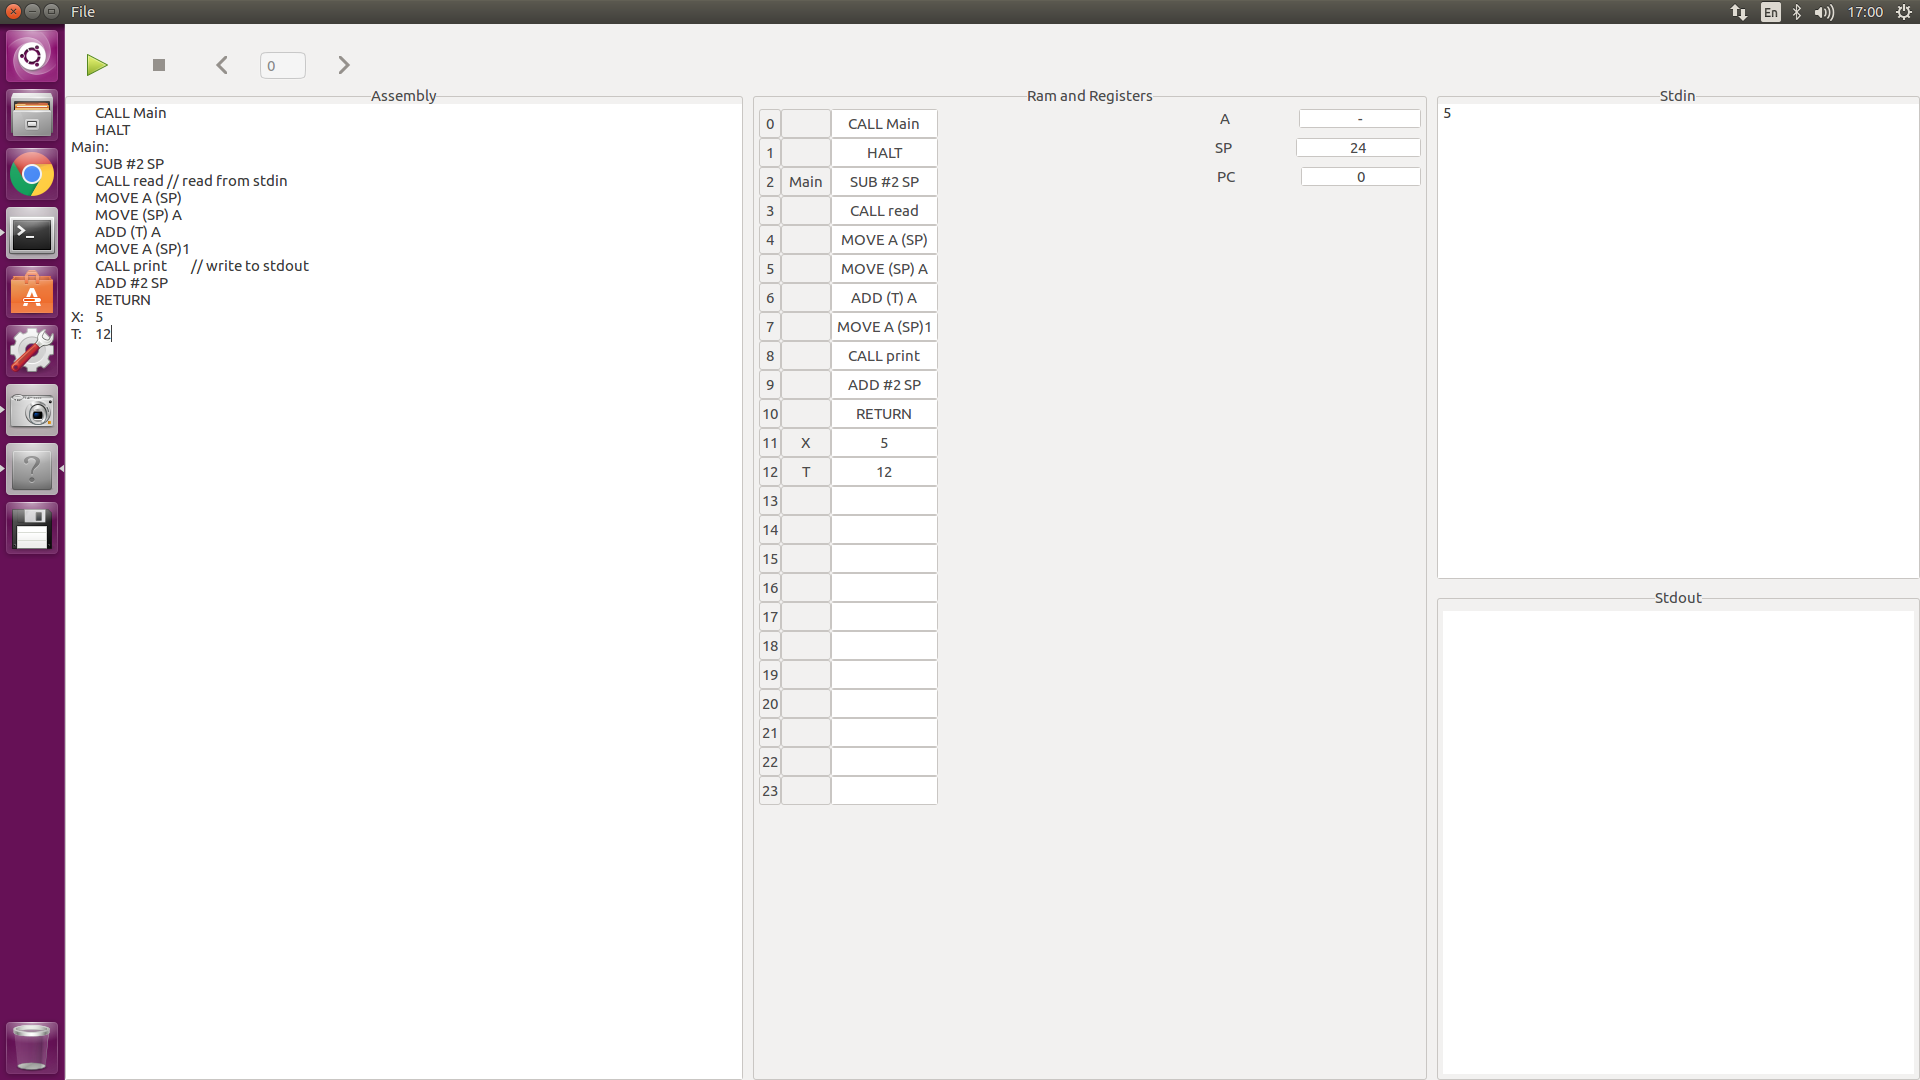
\includegraphics[width=300px]{screen_shot}
    \caption{Screenshot of the Final Product}
    \label{fig:screen_shot}
\end{figure}

\begin{figure}[h]
    \centering
    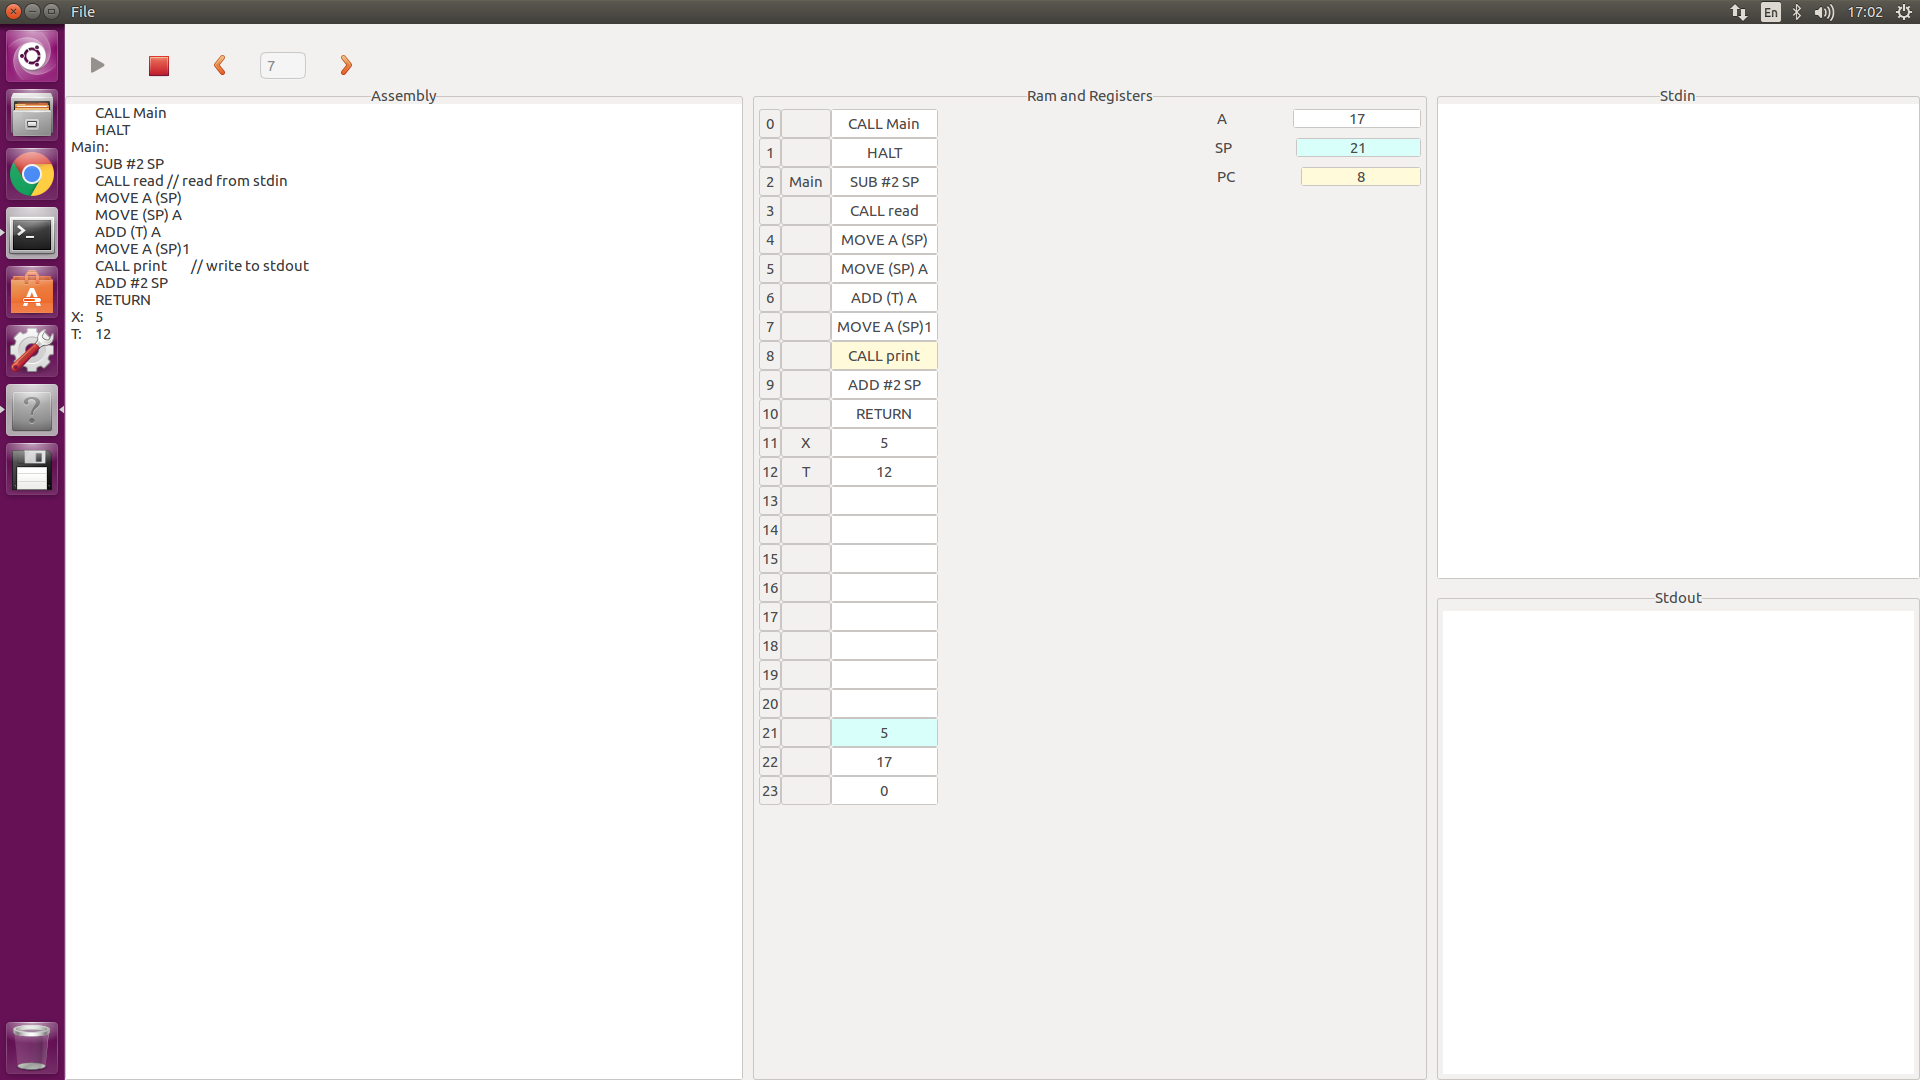
\includegraphics[width=300px]{screen_shot_running}
    \caption{Screenshot of the Final Product Running}
    \label{fig:screen_shot_running}
\end{figure}

\section{Design Details}
Details about the design.
present the grammars, etc - No grammers for our project.

- How to compile the project

\subsection{Compiling on Windows}
Although GTK3 is a cross platform library, getting everything installed on windows to compile it with Haskell is actually quite hard. This tutorial was written based off instructions from multiple websites that were all out of date. 
\linebreak \\
\textbf{Step 1}: Haskell on Windows
I used the Haskell Platform to install haskell on Windows. This provides haskell commands (ghc, cabal etc) through the windows command prompt. (\href{https://www.haskell.org/platform/}{https://www.haskell.org/platform/})

\noindent Though any Haskell installation for windows should work just fine for this.
\linebreak \\
\textbf{Step 2}: Get the GTK3 and Glade Binaries and dependencies
In order to get the up to date gtk3 binaries, and all the dependencies, we need to use msys. Download msys (\href{https://sourceforge.net/projects/msys2/}{https://sourceforge.net/projects/msys2/}) and install to a path without spaces. I installed to C:\\dev\\msys . You could do this without msys, but we need quite a few libraries, and they are not easy to find by themselves and it is not recommended to install them without msys.

Once installed, run msys and you'll get a console, this is what we get all the packages with. First we need to update msys. Type:
Run pacman -Syuu

Then quit the console and open it again.

Now we get the packages. Each package has a 32-bit and 64-bit version. Install the one suitable for you. I was on a 64-bit computer, so I used the 64-bit packages.

\noindent \textbf{pkg-config:}\\
pacman -S mingw-w64-i686-pkg-config    (32-bit)\\
pacman -S mingw-w64-x86\_64-pkg-config  (64-bit)\\

\noindent \textbf{cairo:}\\
pacman -S mingw-w64-i686-cairomm    (32-bit)\\
pacman -S mingw-w64-x86\_64-cairomm  (64-bit)\\

\noindent \textbf{glib:}\\
pacman -S mingw-w64-i686-glib2    (32-bit)\\
pacman -S mingw-w64-x86\_64-glib2  (64-bit)\\

\noindent \textbf{gtk2:}\\
pacman -S mingw-w64-i686-gtk2    (32-bit)\\
pacman -S mingw-w64-x86\_64-gtk2  (64-bit)\\

\noindent \textbf{gtk3:}\\
pacman -S mingw-w64-i686-gtk3    (32-bit)\\
pacman -S mingw-w64-x86\_64-gtk3  (64-bit)\\
\linebreak
\textbf{Step 3}: Haskell packages.
Now that we have all the c libraries, we can install the connected Haskell packages. First we need to link the c libraries so that Haskell can see them. To do this we need to edit a system environment variable.

Go to \verb"Computer -> System Properties ->" \\
\indent \verb"Advanced System Properties -> Environment Variables".

\noindent In the top box you'll see a variable called PATH, edit this. Values are separated by ; so add a ; to the end and then put the filepath to \verb"msys64\mingw64\bin". In my case this was \verb"C:\dev\msys64\mingw64\bin". Now open up a windows command prompt (with administer privileges).

\noindent Now for some Haskell libraries we need install. As always, use:\\
cabal update\\

\noindent Then:\\
cabal install alex\\
cabal install happy\\
cabal install gtk2hs-buildtools\\

\noindent Now it gets harder, there was/is a bug on Windows for a few of the Haskell library. glib, gio, pango and gtk3 all will fail to install directly with cabal. Try to install it first, but if you get an error about \verb"__debugbreak", then you'll have to do some editing.

Navigate to a location where we can unpack each package. I just used \verb"c:\dev\" where I installed msys and the Haskell platform, but the location doesn't matter. Then use cabal unpack to download and unpack the following packages.\\

\noindent cabal unpack glib\\
cabal unpack gio\\
cabal unpack pango\\
cabal unpack gtk\\
cabal unpack gtk3\\

\noindent Now go into each unpacked package and open the .cabal file, remove the \verb"-D__attribute__(A)=" attribute from the cpp-options.
\\ \linebreak

\noindent At the time of writing, there is a bug in gio that will cause this error: \\
\verb"System\GIO\File\IOError.chs:49:15: parse error on input '*'"
\linebreak

\noindent This bug has already been fixed in gtk2hs, but not in gio. You'll need to edit one of the source files. Find \verb"\gio-0.13.1.1\System\GIO\File\IOError.chs" and delete the \verb"{-# LANGUAGE CPP #-}" line. This file does not require cpp, and cpp ends up processing part of a comment, causing the error.
\\ \linebreak

\noindent Now manually install each of these pages, go into each unpacked package with the console and type: \\
cabal install \\
In the same order as when you unpacked them above.
\\ \linebreak

\noindent \textbf{Step 4}: Done \\
You're finally done and should be able to compile this project.

\section{Implementation}
\subsection{Environment}
\input{../Environment.lhs}

\subsection{Emulation}
\input{../Emulation.lhs}

\subsection{GUI}
GTK3 runs everything through a main loop.  Therefore it uses an event-driven paradigm where the program mostly does nothing until certain events are triggered.  The "main loop" is responsible for waiting for user input and invoking the appropriate listener functions.  It is very important to note that the main loop is blocking while it waits for user input.  Therefore you must do everything based on an event.

\section{Results, evidence of what works}
Screenshots of the GUI and output of printing an environment I guess.

\section{Conclusion}

\subsection{Callum McColl's Reflection}

\subsection{Andrew Paroz's Reflection}


\end{document}



